% !TeX encoding = UTF-8
% !TeX spellcheck = es_ES
% !TeX root = ../ComponentCatalog.tex
%!TEX root=../ComponentCatalog.tex

%RCY
\begin{table}[H]
    \centering
    \renewcommand\theadfont{\bfseries}
    \setlength{\tabcolsep}{10pt}
    \renewcommand{\arraystretch}{1.5}

    \begin{tabular}{|c|c|c|c|c|}
        \beginConnectorTable{JST RCY 2 Vias}
        \multirow{5}{*}{\makecell{Macho \\ Plug }}

        \connectordata{
            \begin{scope}
                \clip (0,0) rectangle  +(3,1.5);
                \node[inner sep=0pt] at (-1.9,1.7)
                    {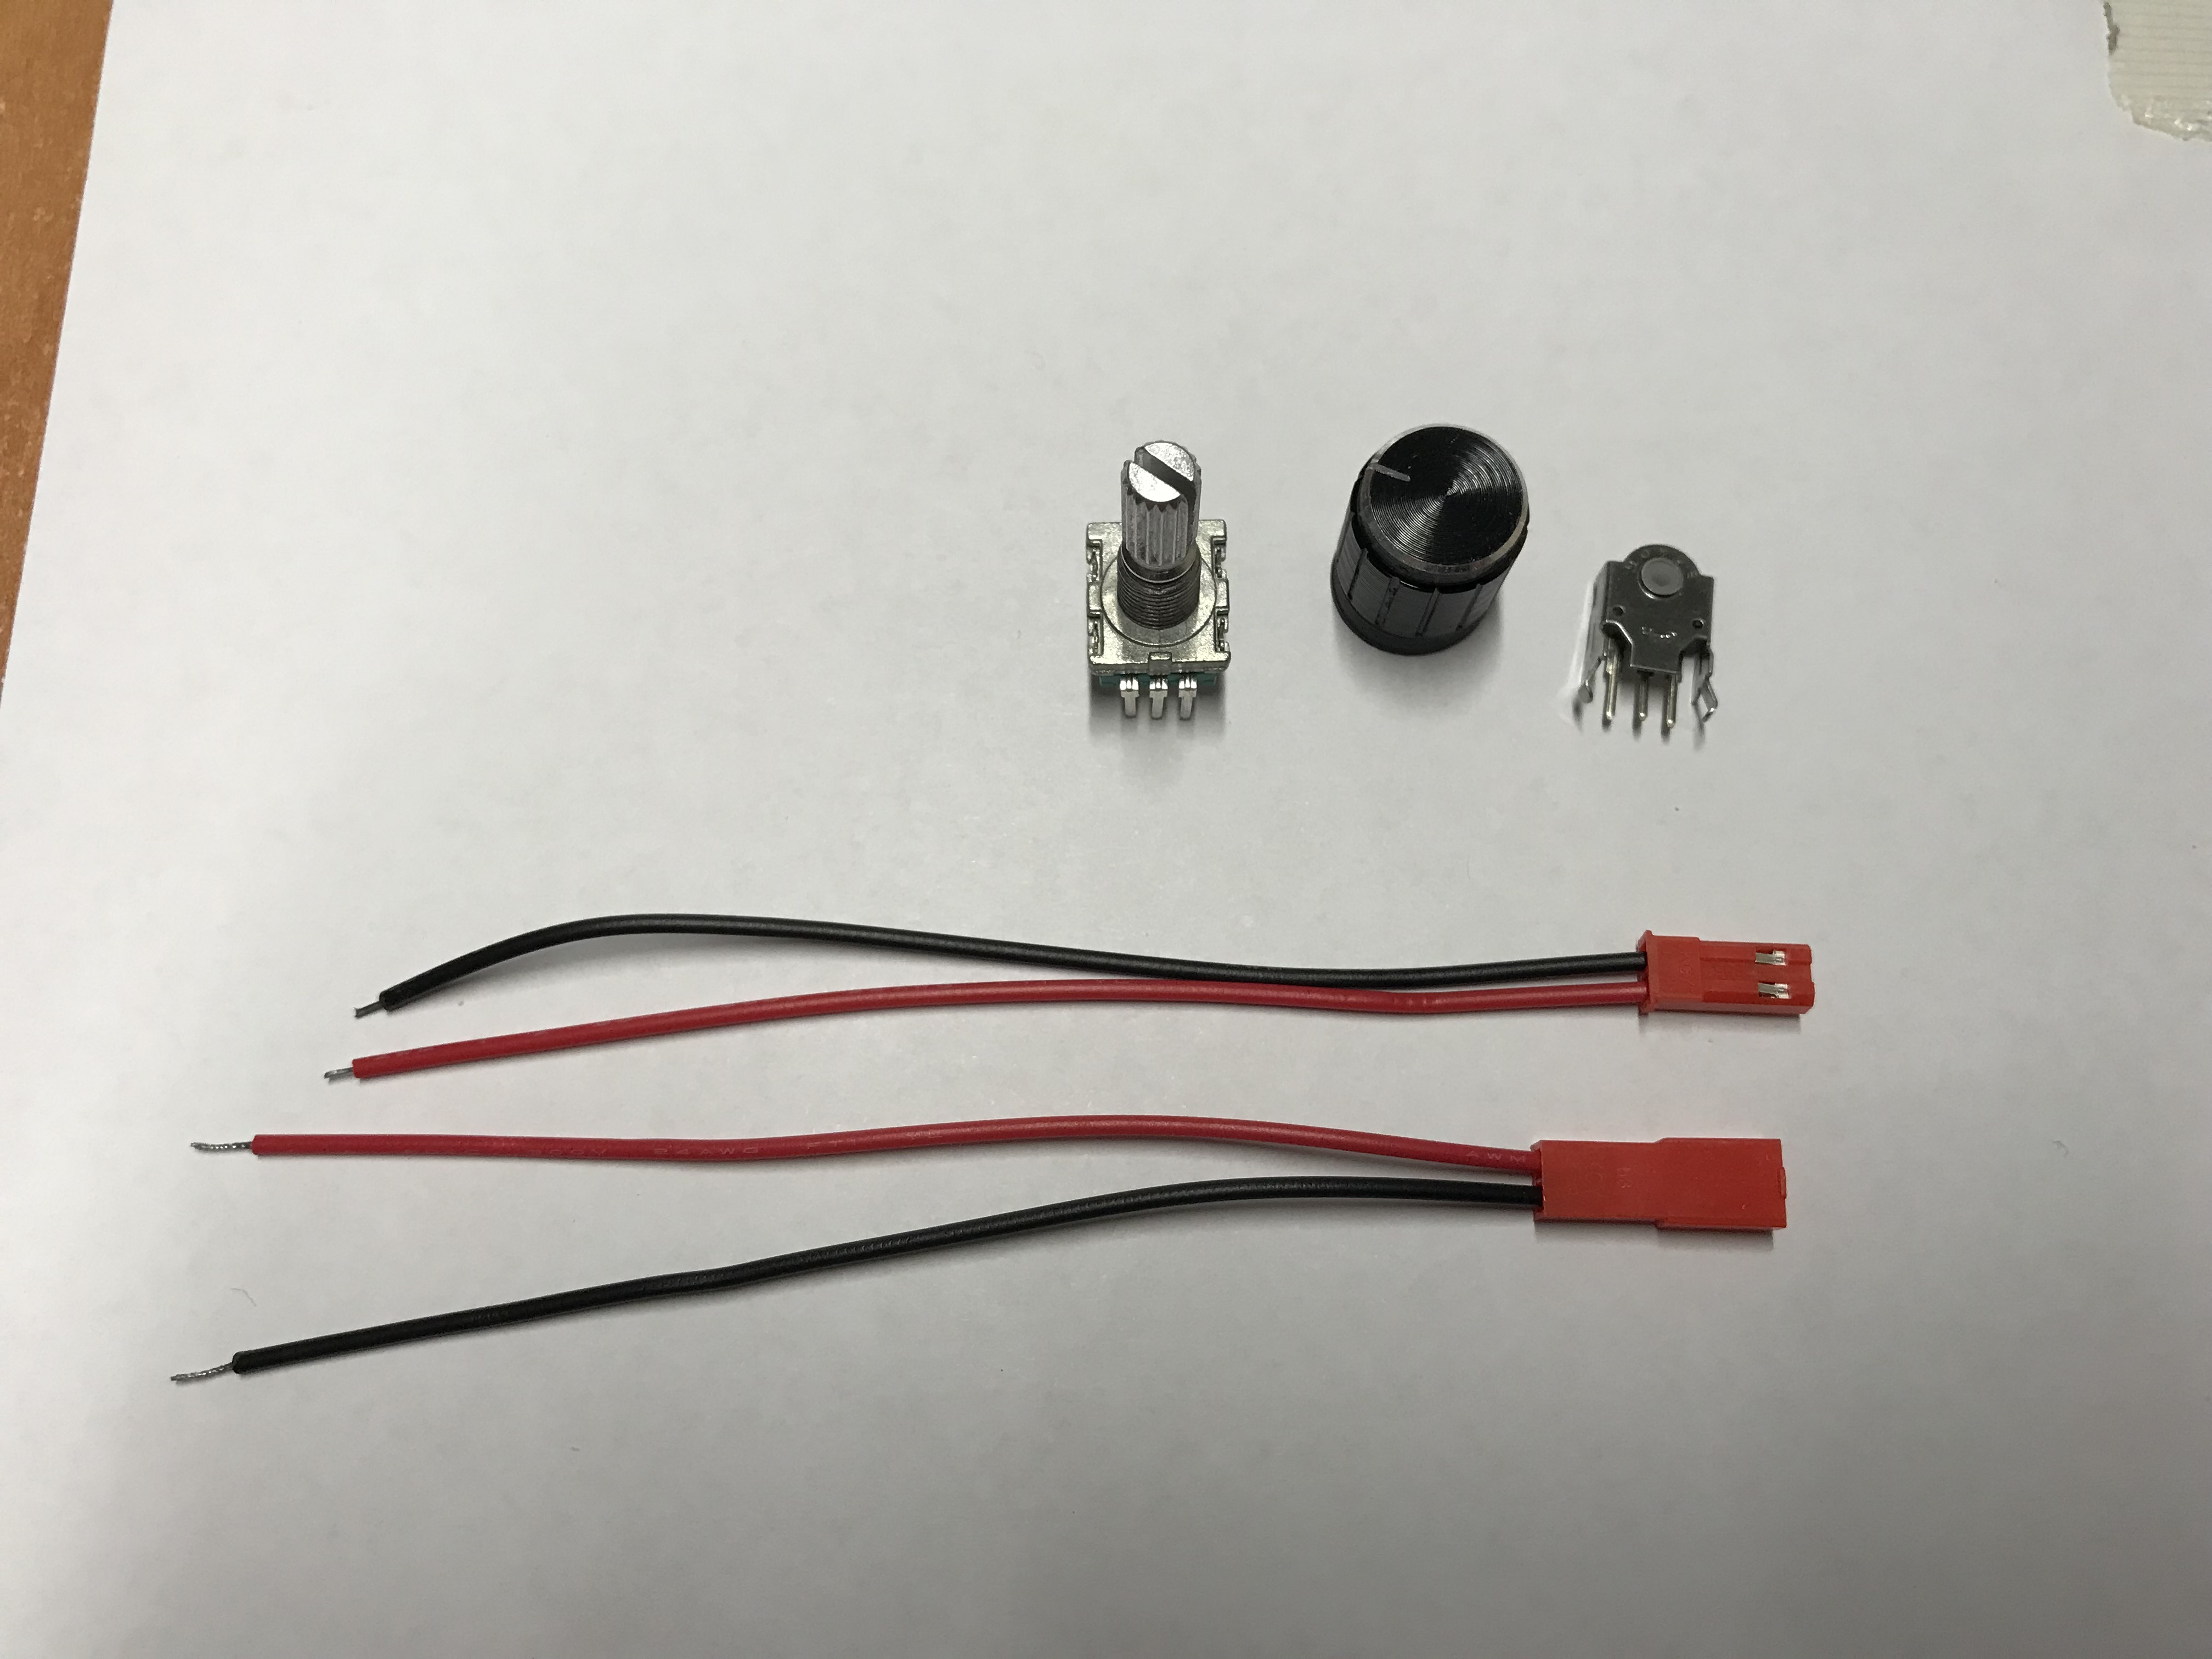
\includegraphics[scale=.1]{pictures/JST.jpg}};
            \end{scope}
        }{
            \draw (0,0) rectangle (3,1.5) ;
        }{Aliexpress}{JST RCY} {250V} {3A} 
        
        \connectorinfo{Housing}{SYP-02T-1}{
            \tabitem \textbf{Tipo}: Plug  \\
             \tabitem \textbf{Color}: Rojo
        }
        \connectorinfo{Contact}{SYF-001T-P0.6}{
            \tabitem \textbf{Tipo}: Socket  \\
            \tabitem \textbf{AWG}: 22-28 \\
            \tabitem \textit{Alternativa}:	BYF-001T-P0.6
        } 
        \cline{1 - 2}

        \multirow{3}{*}{\makecell{Hembra \\ Socket}}
        \connectordata{
            \begin{scope}
                \clip (0,0) rectangle  +(3,1.5);
                \node[inner sep=0pt] at (-1.8,3)
                    {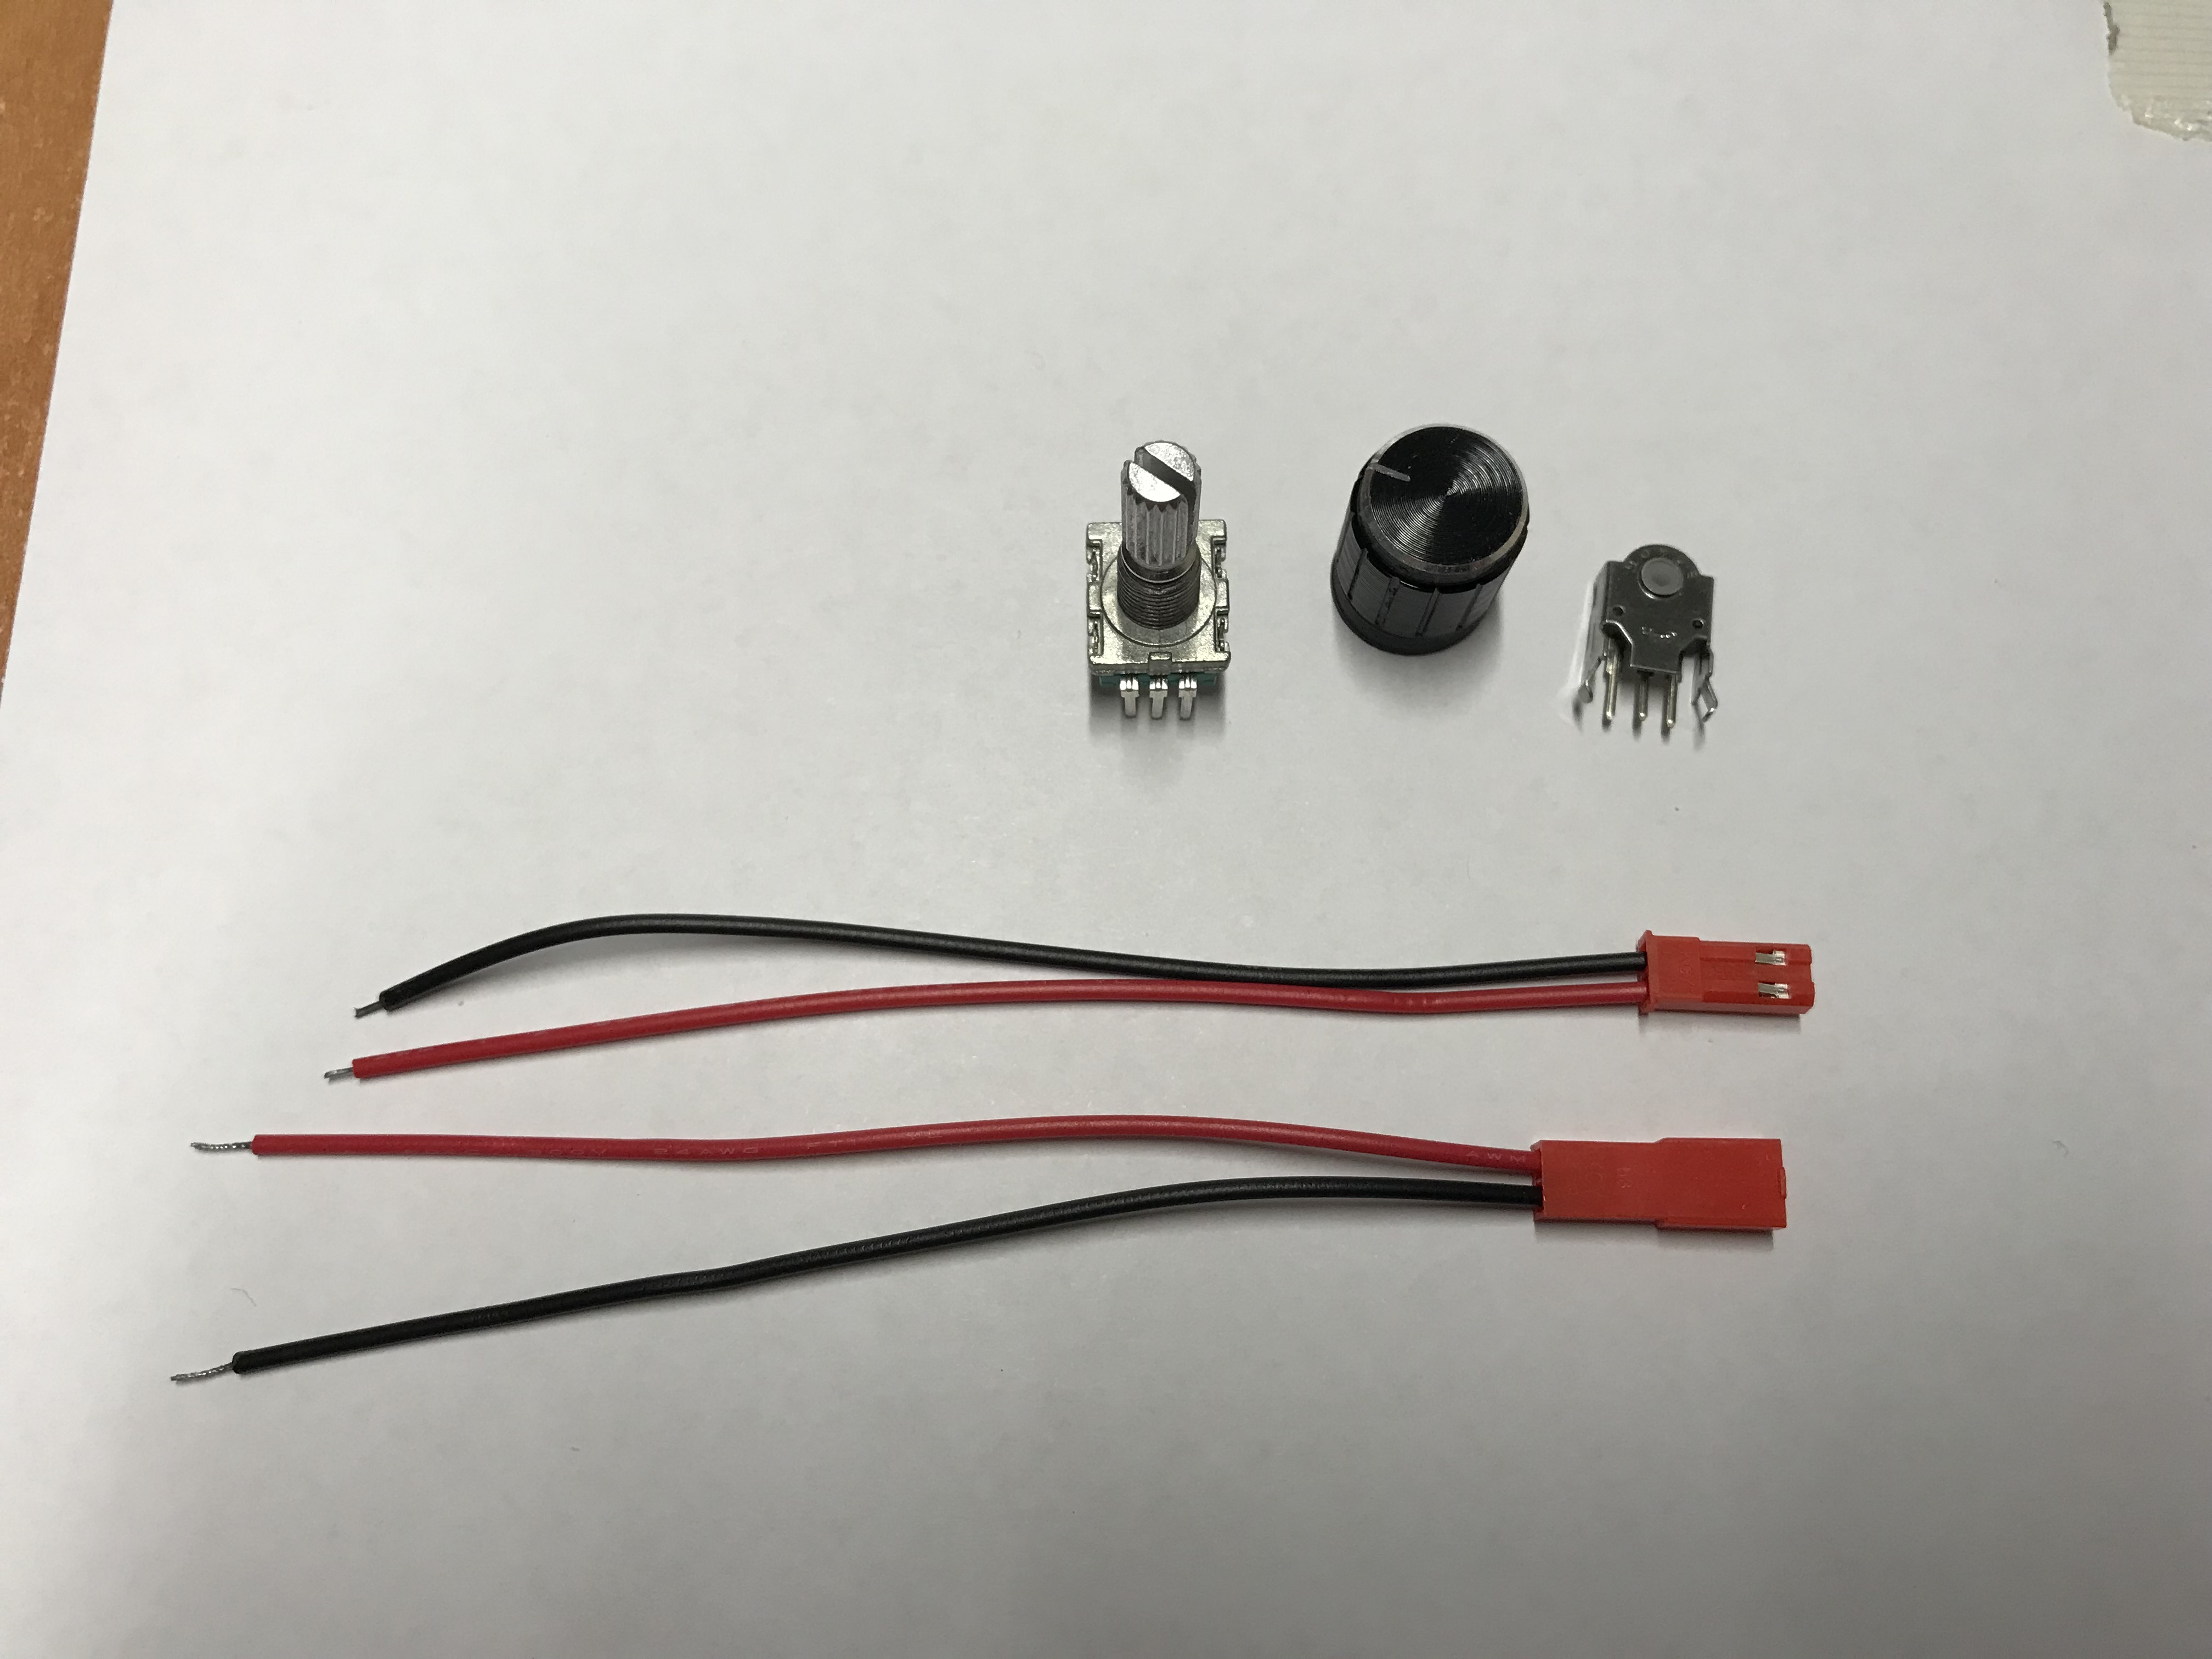
\includegraphics[scale=.1]{pictures/JST.jpg}};
            \end{scope}
        }{
            \draw (0,0) rectangle (3,1.5) ;
        }{Aliexpress}{JST RCY} {250V} {3A}
        \connectorinfo{Housing}{SYR-02T}{
            \tabitem \textbf{Tipo}: Receptacle  \\
             \tabitem \textbf{Color}: Rojo
        }
        \connectorinfo{Contact}{SYM-001T-P0.6}{
            \tabitem \textbf{Tipo}: Pin  \\
            \tabitem \textbf{AWG}: 22-28 \\
            \tabitem \textit{Alternativa}: BYM-001T-P0.6
        }
        \cline{1 - 2}
        \multicolumn{5}{|l|}{\makecell[l]{
            \tabitem Incluyen cables presoldados
        }} \\
        \hline
        \connectorblockinfo{Uso}{Paso de corriente entre modulos}
        \connectorblockinfo{Ubicacion}{TR}
    \end{tabular}
    \caption{JST RCY}
    \label{tab:DcJstRcy}
\end{table}